\title{A 90 Minute \textit{SAGA} Hands-On Tutorial\\[1em]
\Large{ISSGC, Nice, France, July 14 2009 } \\[1em]
\large{Ole Weidner, Hartmut Kaiser, Andre Merzky, Shantenu Jha}}

\documentclass[12pt]{article}

 \usepackage{graphicx}

\usepackage{color}
\newif\ifdraft
\drafttrue
\ifdraft
\newcommand{\amnote}[1]{   {\textcolor{magenta} { ***Andre: #1 }}}
\newcommand{\olenote}[1]{{\textcolor{blue}    { ***Ole: #1 }}}
\newcommand{\hartmutnote}[1]{  {\textcolor{green}     { ***Hartmut:    #1 }}}
\newcommand{\jhanote}[1]{  {\textcolor{red}     { ***Shantenu:    #1 }}}
 \usepackage[pdftex,colorlinks=true, linkcolor=blue,citecolor=blue,
       urlcolor=blue]{hyperref}
\else
\newcommand{\amnote}[1]{}
 \newcommand{\olenote}[1]{}
\newcommand{\note}[1]{}
\newcommand{\hartmutnote}[1]{}
 \newcommand{\jhanote}[1]{}
\fi
\begin{document}

\maketitle

%\begin{abstract}
%This is the paper's abstract \ldots
%t\end{abstract}

\section*{Scope of this Tutorial}
The scope of this tutorial is to provide the audience with the required resources and technical knowledge (hands-on experience) to start hacking their own distributed applications with SAGA.

\subsection*{Prerequisites} This tutorial requires basic knowledge of the C/C++ programming language. Experience using the command line on a Linux/UNIX based operating system and a basic idea of what a compiler, a linker and a Makefile is might come in handy.\\[0.4em]
Unless this tutorial is going to be preceded by a SAGA installation tutorial, the students are required to have a fully working installation of SAGA on their laptops/lab machines (preferred), or remote access (e.g. via SSH) to a machine with SAGA installed.
	
%\subsection*{Cheat Sheat} At the beginning of the tutorial we're going to hand out the SAGA Cheat Sheet (yet to be %created). The cheat sheet is a double-sided % (laminated, so people won't throw it away!)
%letter-sized piece of paper with hints and tips for writing, compiling, and running SAGA applications.

\subsection*{ISSGC Infrastructure}

\begin{figure}[!ht]
  \begin{center}
      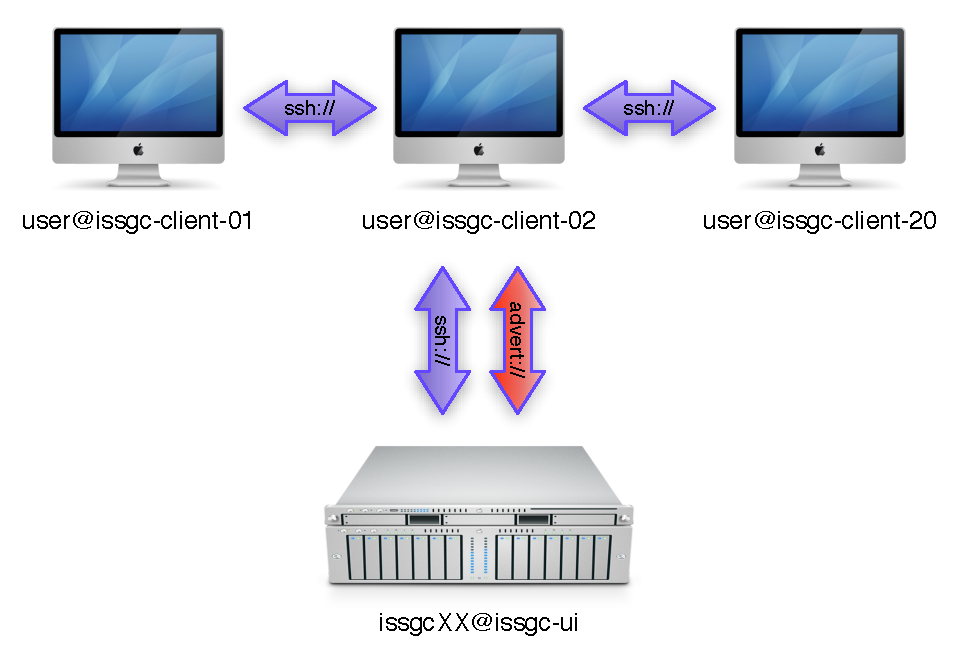
\includegraphics[width=1\textwidth]{infrastructure}
 \end{center}
\end{figure}


The summer school infrastructure consists of a set of client machines issgc-client-01 to issgc-client-20 and a server issgc-ui. Since SAGA provides a uniform API for job submission, it doesn't make a difference to the wether you submit your jobs through gLite, Globus, Condor or any other middleware. For the sake of simplicity, we set up the machines with SSH in a way that allows you to submit "jobs" to any other client or the server and transfer data between all available machines. Before you start using SAGA, please make sure that SSH work on your lab machine:

\begin{verbatim}
ssh user@issgc-client-XX /bin/hostname
ssh issgcXX@issgc-ui /bin/hostname
\end{verbatim}

Remember these host names. You will use them again in your SAGA program in the form of:

\begin{verbatim}
saga::url my_resource("ssh://user@issgc-client-XX");
saga::url my_other_resource("ssh://issgcXX@issgc-ui");
\end{verbatim}

The server also hosts a SAGA advert DB (PostgreSQL). You will use it in one of the exercises to
store some data. To make sure that you don't mess with each other's data, we created directories
for each participant - make sure that you can access yours:

\begin{verbatim}
source /opt/saga-1.3.1-issgc/share/saga/saga-env.sh
saga-advert list_directory advert://issgc-ui//issgcXX/ ?
\end{verbatim}

\subsection*{Unit I (15 min)} \textbf{SAGA Applications:} Every application that uses just a single SAGA call is considered a SAGA application, since it triggers the whole (SAGA) stack. SAGA is not a framework, but it provides the building blocks from which to develop frameworks or applications; loosly speaking, SAGA is programming system, but it does not impose a specific programming model.  Remember the rough taxonomy that we presented of three ways of developing applications using SAGA: (i) Implement a distributed submission/execution mode for a {\it legacy} application; (ii) Create a framework that supports a specific application characteristics and/or pattern, or (iii) Compose applications from multiple (distributed) units, which in a way makes it an {\it a priori} application.

%Look at it as a TOOLBOX for distributed computing.
%\jhanote{Remember, we are going to use SSH adaptors for everything and nothing will USE Globus}

\begin{verbatim}
<CODE>
\end{verbatim}

\jhanote{Points/Issues to consider here: (i) Avoid Context, (ii) Copy a file given 2 URLS, and (iii) Command line Tools. Make Use of material already in the programming manual}

\begin{verbatim}
#include <saga/saga.hpp>

int main(int argc, char * argv[]) 
{
  saga::url source("ssh://issgc12@issgc-ui//etc/passwd");
  saga::url target(".");
  
  saga::filesystem::file file (source, saga::filesystem::Read);
  file.copy(target);

  return 0;
}
\end{verbatim}

\subsection*{Unit II (15 min)} \textbf{Compiling and linking.} Like with any other C/C++ library, you have to let the 
compiler and the linker know where to find the header files and the library. To make life easier, SAGA provides
a Makefile which you can include in order to build your application:

\begin{verbatim}
SAGA_SRC          = $(wildcard *.cpp) 
SAGA_ADD_BIN_OBJ  = $(SAGA_SRC:%.cpp=%.o) 
SAGA_BIN          = my_saga_app 

include $(SAGA_LOCATION)/share/saga/make/saga.application.mk 

## Other (optional) compiler and linker flags 
SAGA_CPPFLAGS    += -I/opt/super/include 
SAGA_LDFLAGS     += -L/opt/super/lib -lsuper 
\end{verbatim}

Of course it's also possible to compile and link a SAGA application manually:

\begin{verbatim}
g++ -Wall -I/opt/saga-1.3.1-issgc/include -pthread \ 
    -L/opt/saga-1.3.1-issgc/lib \
    -lsaga_engine -lsaga_package_job -lsaga_package_XYZ \
    <FILENAME>.cpp

\end{verbatim}

\subsection*{Unit III (15 min)} \textbf{Running a SAGA application.}
Explain what needs to be in the loader path. Explain the effects of SAGA\_VERBOSE and how it can be used to debug a saga application. Demonstrate how the engine launches adaptor loading, etc... in the background.

\begin{verbatim}
<CODE>
\end{verbatim}

\section*{Unit IV (20 min)}\textbf{SAGA-based Applications:}
In this tutorial, we will work with three different examples. The aim of these
applications is to give you a  quick feel for how SAGA is actually utilized to develop distributed applications. And although these examples are by definition very simple, they are representative of the way you would use SAGA in a real world examples to develop many of the scientific applications you heard about in today's 
lecture such as Replica-Exchange and C0$_2$ Sequestration problem(s).

In the first example, we will introduce a simple ``Hello Distributed World!'', where the aim will be to submit three simple remote jobs using SAGA. In the second example application (``chaining\_jobs.cpp''), we will serialize the launch of three (remote) jobs, so that the second job is launched after the first, and the third job is launched after the second. In the third example application (``depending\_jobs.cpp''), we will start an application that once started, is able to re-spawn itself on another machine and after doing so increments a ``global counter''. Finally, we will leave you with a programming excercise that will build upon your understanding of application examples 2 and 3.

\subsection*{Example 1: Hello distributed world!} Submit three jobs to three machines. One returns �Hello�, one returns �Distributed� and one returns �World�. They may or may not return in the right order. This should give the student an idea how they could potentially speed up their application using multiple resources. 


\begin{verbatim}
// The hello_world example is meant to be a very simple and first example to 
// try when it comes to SAGA. It's purpose is to spawn 3 (possibly remote) 
// identical jobs (/bin/echo) while passing the 3 words "Hello", "distributed", 
// and "world!" on their command lines. The result is that the jobs will print
// the respective command line arguments (hey, it's /bin/echo we're 
// launching...). The master job (this one) waits for the 3 child jobs to 
// finish. It intercepts the generated output and prints it to the user.
//
// Depending on which child jobs finish first the overall printed message might
// be some combination of the 3 arguments we passed. But most of the time you
// will see "Hello distributed world!", which is our way of saying hello and
// welcome to the world of SAGA.


// the routine spawning the SAGA jobs and waiting for their results
void run_a_job(std::string host, std::string argument)
{
    try {
        saga::job::service js (host);
        saga::job::ostream in;
        saga::job::istream out;
        saga::job::istream err;

        // run the job
        saga::job::job j = js.run_job("/bin/echo " + argument, host, in, out, err);

        // wait for the job to finish
        saga::job::state s = j.get_state();
        while (s != saga::job::Done && s != saga::job::Failed)
            s = j.get_state();

        // if the job finished successfully, print the generated output
        if (s == saga::job::Done) {
            std::string line;
            while (!std::getline(out, line).eof())
                std::cout << line << '\n';
        }
        else {
            std::cerr << "SAGA job: " << j.get_job_id() << " failed (state: " 
                      << saga::job::detail::get_state_name(s) << ")\n";
        }
    }

   catch (saga::exception const& e) {
        std::cerr << "saga::exception caught: " << e.what () << std::endl;
    }
    catch (std::exception const& e) {
        std::cerr << "std::exception caught: " << e.what () << std::endl;
    }
    catch (...) {
        std::cerr << "unexpected exception caught" << std::endl;
    }
}

///////////////////////////////////////////////////////////////////////////////
int main(int argc, char* argv[])
{
    // run 3 separate threads executing the saga calls
    boost::thread t1 (run_a_job, HOST1, "Hello");
    boost::thread t2 (run_a_job, HOST2, "distributed");
    boost::thread t3 (run_a_job, HOST3, "world!");

    // wait for all spawned threads to finish
    t1.join();
    t2.join();
    t3.join();
    return 0;
}

\end{verbatim}

\subsection*{Example 2: Multiple Sequential Jobs} \textbf{Applications} The aim of this section is to see how SAGA is used to implement common {\it higher-level} functionality that is used by Distributed Applications (DA). Specifically, we will look at two commonly occuring functionality required by DA.

{\bf Example 1:} Here we will demonstrate the ability to checkpoint, use a specified resource, self-migrate and restart on a different computational resource. There are multiple reasons this might be required (see lecture notes). Here we will demonstrate this capability using the \textbf{Hello distributed world!} example discussed in Unit IV.  Instead of launching three jobs on three machines, we will launch one job on one machine, which will then launch itself on another machine, which in turn will do so onto yet another machine. 

\begin{verbatim}
//////////////////////////////////////////////////////////////////////////////
// The chaining_jobs example tries to overcome one of the limitations of the 
// hello_world example: it introduces dependencies between 3 (possibly remotely)
// spawned childs. In this example the next child will be spawned only after 
// the previous one has finished its execution. To make it more interesting we 
// now use /usr/bin/bc to do some calculations, where the result of the previous
// calculation is used as the input for the next one.
//
// Try to make more complex calculations if you like!
///////////////////////////////////////////////////////////////////////////////

///////////////////////////////////////////////////////////////////////////////
// the routine spawning the SAGA jobs and waiting for their results
std::string increment(std::string host, std::string argument)
{
    try {
        saga::job::service js (host);
        saga::job::ostream in;
        saga::job::istream out;
        saga::job::istream err;

        // run the job
        saga::job::job j = js.run_job("/usr/bin/bc -q", host, in, out, err);

        // wait for the job to finish
        saga::job::state s = j.get_state();
        while (s != saga::job::Running && s != saga::job::Failed)
            s = j.get_state();

        // if the job didn't start successfully, print error message
        if (s == saga::job::Failed) {
            std::cerr << "SAGA job: " << j.get_job_id() << " failed (state: " 
                      << saga::job::detail::get_state_name(s) << ")\n";
            return argument;
        }

        // feed the remote process some input
        in << "1 + " + argument + "\n";

        // receive result
        std::string line;
        std::getline(out, line);

        // quit remote process
        in << "quit\n";

        return line;
    }
    catch (saga::exception const& e) {
        std::cerr << "saga::exception caught: " << e.what () << std::endl;
    }
    catch (std::exception const& e) {
        std::cerr << "std::exception caught: " << e.what () << std::endl;
    }
    catch (...) {
        std::cerr << "unexpected exception caught" << std::endl;
    }
    return argument;    // by default just return argument
}

///////////////////////////////////////////////////////////////////////////////
int main(int argc, char* argv[])
{
    // run 3 separate threads executing the saga calls
    std::string result = increment(HOST1, "1");
    result = increment(HOST2, result);
    result = increment(HOST3, result);

    std::cout << "The overall result is: " << result << std::endl;

    return 0;
}

\end{verbatim}

Once developed, this capability can be utilized by a wide range of different applications. In other words this capability described/shown above is independent of any specific application logic. Do you know of a (Scientific) application that could utilize this feature?

\subsection*{Example 3: Managing Dependies between Jobs}

In this example, we will introduce the {\it advert service} as a simple mechanism to provide coordination between different distributed tasks.  Specifically, the advert service will be used by a set of jobs to increment a global counter everytime a job is successfully spawned. There are other ways of {\it coordinating} distributed tasks/jobs, but the idea of a centralized data-store is arguably the simplest, even if not the most robust (fault-tolerant) or tuned for performance.


\begin{verbatim}

///////////////////////////////////////////////////////////////////////////////
// Start this example by providing an arbitrary number of hosts on the command 
// line. It will re-spawn itself on each of the hosts. Each instance will 
// increment a number stored in a central result store.

///////////////////////////////////////////////////////////////////////////////


///////////////////////////////////////////////////////////////////////////////
// the routine spawning the SAGA jobs and waiting for their results
void respawn(int argc, char *argv[])
{
    assert(argc > 1);     // we shouldn't end up here without any given hosts
    try {
        saga::job::service js (argv[1]);

        // compose the command line, skip first argument
        std::string commandline (JOB_PATH);
        for (int i = 2; i < argc; ++i) {
            commandline += " ";
            commandline += argv[i];
        }

        // run the job on host given by first argument
        saga::job::job j = js.run_job(commandline, argv[1]);

        // wait for the job to start
        saga::job::state s = j.get_state();
        while (s != saga::job::Running && s != saga::job::Failed)
            s = j.get_state();

        // if the job didn't start successfully, print error message
        if (s == saga::job::Failed) {
            std::cerr << "SAGA job: " << j.get_job_id() << " failed (state: " 
                      << saga::job::detail::get_state_name(s) << ")\n";
        }

        // wait for the job to Finish
        s = j.get_state();
        while (s == saga::job::Running)
            s = j.get_state();
    }

    catch (saga::exception const& e) {
        std::cerr << "saga::exception caught: " << e.what () << std::endl;
    }
    catch (std::exception const& e) {
        std::cerr << "std::exception caught: " << e.what () << std::endl;
    }
    catch (...) {
        std::cerr << "unexpected exception caught" << std::endl;
    }
}

///////////////////////////////////////////////////////////////////////////////
int main(int argc, char* argv[])
{
    if (argc == 1) {
    // no more hosts are given, we're done!
        int result = 0;
        if (get_result(result))
            std::cout << "The overall result is: " << result << std::endl;
    }
    else {
    // otherwise get current value, increment it, and store new value
        int result = 0;
        get_result(result);   // ignore errors, will set result to zero

        // re-spawn this job, increment result
        if (set_result(result + 1)) 
            respawn(argc, argv);
    }
    return 0;
}

\end{verbatim}

{\bf A Real World Example} Here we will briefly discuss MapReduce -- a computational pattern made famous by Google's use for its Search Engine Infrastructure.  The fundamental idea is that there is a Master which coordinates the distribution of work to a large number of Workers, and manages the merging of the output of the computation that the Workers produce. In addition to performance, a fundamental challenge is the need to be able to coordinate Master-Workers across a wide range of distributed systems.

\begin{verbatim}
<CODE>
\end{verbatim}

Not surprisingly the code snippet above is independent of any application specific details and focusses on the assignment of workloads to workers, execution and then retrival. This specific approach adopted here relies heavily on the use of the Advert Service.  Although introduced in the context of MapReduce, the requirement of coordination of distributed, often heteregenous units is a fundamental {\it vector} of distributed applications. (See Lecture Notes).


\subsection*{Programming Excercise:} 

In earlier examples, we introduced the underlying concepts of submitting jobs and coordination amongst multiple distributed jobs (tasks), where we updated the value of a counter. Can the same approach (i.e. advert) be used to coordinate the submission of multiple jobs? In effect, this is a way of informing a job (that is ready to spawn another job) about which (possible) machines to spawn too.
The aim of this excercise is for you to complete the code by implementing
some (i) job submission functionality, and (ii) accessing advert entries.
(We will post a sample solution to this at the end of the tutorial).

\begin{verbatim}
<CODE>
\end{verbatim}

Think of generalizations to this concept: Say one application is ``producing'' this information (that is a list of possible resources), and this information is being ``consumed'' by another application.

\subsection*{Conclusion}

Let us recap that there are multiple types of distributed applications. What you have seen here are simple applications that utilize distributed functionality, such as remote job submission to achieve tasks.  What you should take away from this tutorial are essentially the following: 

\begin{itemize}

\item Distributed Applications can be developed much like regular applications.  The challenges facing Distributed Applications -- development and deployment are different from traditional applications and many of those challenges arise from the distributed infrastructure. It is to precisely meet these ``unique'' distributed computing challenges that there is a need for simple, standard and pervasive
application level interface such as SAGA was conceived.

\item We have focussed on some of the challenges of developing distributed applications, such as coordinating distributed tasks. We have shown the ability to do so in a simple fashion; however this is not necessarily scalable, and poses challenges for many real-world applications. Some other real-world challenges we have not discussed here are fault-tolerance, recovery, replication etc. SAGA provides APIs to these ``Advanced'' features as well.

\item Interestingly, we have built all the distributed functionality around simple ``ssh'' adaptors; if you wanted to launch to a Globus or a Condor specific infrastructure, you would just configure SAGA to utilize Globus or Condor specific adaptors. 

\item All of these exist in the full SAGA installation (http://saga.cct.lsu.edu is your source of information for all things SAGA).

\end{itemize}

\end{document}
